% Template for PLoS
% Version 3.4 January 2017
%
% % % % % % % % % % % % % % % % % % % % % %
%
% -- IMPORTANT NOTE
%
% This template contains comments intended
% to minimize problems and delays during our production
% process. Please follow the template instructions
% whenever possible.
%
% % % % % % % % % % % % % % % % % % % % % % %
%
% Once your paper is accepted for publication,
% PLEASE REMOVE ALL TRACKED CHANGES in this file
% and leave only the final text of your manuscript.
% PLOS recommends the use of latexdiff to track changes during review, as this will help to maintain a clean tex file.
% Visit https://www.ctan.org/pkg/latexdiff?lang=en for info or contact us at latex@plos.org.
%
%
% There are no restrictions on package use within the LaTeX files except that
% no packages listed in the template may be deleted.
%
% Please do not include colors or graphics in the text.
%
% The manuscript LaTeX source should be contained within a single file (do not use \input, \externaldocument, or similar commands).
%
% % % % % % % % % % % % % % % % % % % % % % %
%
% -- FIGURES AND TABLES
%
% Please include tables/figure captions directly after the paragraph where they are first cited in the text.
%
% DO NOT INCLUDE GRAPHICS IN YOUR MANUSCRIPT
% - Figures should be uploaded separately from your manuscript file.
% - Figures generated using LaTeX should be extracted and removed from the PDF before submission.
% - Figures containing multiple panels/subfigures must be combined into one image file before submission.
% For figure citations, please use "Fig" instead of "Figure".
% See http://journals.plos.org/plosone/s/figures for PLOS figure guidelines.
%
% Tables should be cell-based and may not contain:
% - spacing/line breaks within cells to alter layout or alignment
% - do not nest tabular environments (no tabular environments within tabular environments)
% - no graphics or colored text (cell background color/shading OK)
% See http://journals.plos.org/plosone/s/tables for table guidelines.
%
% For tables that exceed the width of the text column, use the adjustwidth environment as illustrated in the example table in text below.
%
% % % % % % % % % % % % % % % % % % % % % % % %
%
% -- EQUATIONS, MATH SYMBOLS, SUBSCRIPTS, AND SUPERSCRIPTS
%
% IMPORTANT
% Below are a few tips to help format your equations and other special characters according to our specifications. For more tips to help reduce the possibility of formatting errors during conversion, please see our LaTeX guidelines at http://journals.plos.org/plosone/s/latex
%
% For inline equations, please be sure to include all portions of an equation in the math environment.  For example, x$^2$ is incorrect; this should be formatted as $x^2$ (or $\mathrm{x}^2$ if the romanized font is desired).
%
% Do not include text that is not math in the math environment. For example, CO2 should be written as CO\textsubscript{2} instead of CO$_2$.
%
% Please add line breaks to long display equations when possible in order to fit size of the column.
%
% For inline equations, please do not include punctuation (commas, etc) within the math environment unless this is part of the equation.
%
% When adding superscript or subscripts outside of brackets/braces, please group using {}.  For example, change "[U(D,E,\gamma)]^2" to "{[U(D,E,\gamma)]}^2".
%
% Do not use \cal for caligraphic font.  Instead, use \mathcal{}
%
% % % % % % % % % % % % % % % % % % % % % % % %
%
% Please contact latex@plos.org with any questions.
%
% % % % % % % % % % % % % % % % % % % % % % % %

\documentclass[10pt,letterpaper]{article}
\usepackage[top=0.85in,left=2.75in,footskip=0.75in]{geometry}

% amsmath and amssymb packages, useful for mathematical formulas and symbols
\usepackage{amsmath,amssymb}

% Use adjustwidth environment to exceed column width (see example table in text)
\usepackage{changepage}

% Use Unicode characters when possible
\usepackage[utf8x]{inputenc}

% textcomp package and marvosym package for additional characters
\usepackage{textcomp,marvosym}

% cite package, to clean up citations in the main text. Do not remove.
\usepackage{cite}

% Added natbib for citet commands:
\usepackage{natbib}

% Added url for urls:
\usepackage{url}

% Use nameref to cite supporting information files (see Supporting Information section for more info)
\usepackage{nameref,hyperref}

% line numbers
\usepackage[right]{lineno}

% ligatures disabled
\usepackage{microtype}
\DisableLigatures[f]{encoding = *, family = * }

% color can be used to apply background shading to table cells only
\usepackage[table]{xcolor}

% array package and thick rules for tables
\usepackage{array}

% create "+" rule type for thick vertical lines
\newcolumntype{+}{!{\vrule width 2pt}}

% create \thickcline for thick horizontal lines of variable length
\newlength\savedwidth
\newcommand\thickcline[1]{%
  \noalign{\global\savedwidth\arrayrulewidth\global\arrayrulewidth 2pt}%
  \cline{#1}%
  \noalign{\vskip\arrayrulewidth}%
  \noalign{\global\arrayrulewidth\savedwidth}%
}

% \thickhline command for thick horizontal lines that span the table
\newcommand\thickhline{\noalign{\global\savedwidth\arrayrulewidth\global\arrayrulewidth 2pt}%
\hline
\noalign{\global\arrayrulewidth\savedwidth}}


% Remove comment for double spacing
%\usepackage{setspace}
%\doublespacing

% Text layout
\raggedright
\setlength{\parindent}{0.5cm}
\textwidth 5.25in
\textheight 8.75in

% Bold the 'Figure #' in the caption and separate it from the title/caption with a period
% Captions will be left justified
\usepackage[aboveskip=1pt,labelfont=bf,labelsep=period,justification=raggedright,singlelinecheck=off]{caption}
\renewcommand{\figurename}{Fig}

% Use the PLoS provided BiBTeX style
\bibliographystyle{plos2015}

% Remove brackets from numbering in List of References
\makeatletter
\renewcommand{\@biblabel}[1]{\quad#1.}
\makeatother

% Leave date blank
\date{}

% Header and Footer with logo
\usepackage{lastpage,fancyhdr,graphicx}
\usepackage{epstopdf}
\usepackage{hyperref}% http://ctan.org/pkg/hyperref
\pagestyle{myheadings}
\pagestyle{fancy}
\fancyhf{}
\setlength{\headheight}{27.023pt}
\lhead{
\includegraphics[width=2.0in]{PLOS-submission.eps}}
\rfoot{\thepage/\pageref{LastPage}}
\renewcommand{\footrule}{\hrule height 2pt \vspace{2mm}}
\fancyheadoffset[L]{2.25in}
\fancyfootoffset[L]{2.25in}
\lfoot{\sf PLOS}

%% Include all macros below

\newcommand{\lorem}{{\bf LOREM}}
\newcommand{\ipsum}{{\bf IPSUM}}

%% END MACROS SECTION

\graphicspath{{./figs/}}

\begin{document}
\vspace*{0.2in}

% Title must be 250 characters or less.
\begin{flushleft}
{\Large
\textbf\newline{Hub connectivity and gene expression in the worm connectome} % Please use "sentence case" for title and headings (capitalize only the first word in a title (or heading), the first word in a subtitle (or subheading), and any proper nouns).
}
\newline
% Insert author names, affiliations and corresponding author email (do not include titles, positions, or degrees).
\\
Aurina Arnatkevi\u{c}i\={u}t\.{e}\textsuperscript{1\Yinyang},
Ben D. Fulcher\textsuperscript{1\Yinyang},
Alex Fornito\textsuperscript{1}\\
\bigskip
\textbf{1} Brain and Mental Health Laboratory, Monash Institute of Cognitive and Clinical Neurosciences, School of Psychological Sciences, Monash University, 770 Blackburn Rd, Clayton, 3168, VIC, Australia.
\\
\bigskip

% Insert additional author notes using the symbols described below. Insert symbol callouts after author names as necessary.
%
% Remove or comment out the author notes below if they aren't used.
%
% Primary Equal Contribution Note
\Yinyang These authors contributed equally to this work.

% Additional Equal Contribution Note
% Also use this double-dagger symbol for special authorship notes, such as senior authorship.
% \ddag These authors also contributed equally to this work.

% Current address notes
% \textcurrency Current Address: Dept/Program/Center, Institution Name, City, State, Country % change symbol to "\textcurrency a" if more than one current address note
% \textcurrency b Insert second current address
% \textcurrency c Insert third current address

% Deceased author note
% \dag Deceased

% Group/Consortium Author Note
% \textpilcrow Membership list can be found in the Acknowledgments section.

% Use the asterisk to denote corresponding authorship and provide email address in note below.
* correspondingauthor@institute.edu

\end{flushleft}
% Please keep the abstract below 300 words
\section*{Abstract}
Text


% Please keep the Author Summary between 150 and 200 words
% Use first person. PLOS ONE authors please skip this step.
% Author Summary not valid for PLOS ONE submissions.
\section*{Author summary}
Text

\linenumbers

% Use "Eq" instead of "Equation" for equation citations.
\section*{Introduction}

\begin{enumerate}
    \item{Structural network properties}
    \begin{itemize}
    \item{rich-club, hubs, conservation cross-scale/species/methods}
    \item{Prior work in worm: different types of connectomes - wired/unwired, hubs}
    \end{itemize}

    \item{Structure-expression}
    \begin{itemize}
    \item{Datasets in different scales: mouse/rat, human (also heritability), developmental, large-scale datasets}
    \item{Kaufman example \cite{Kaufman2006}, Baruch 2008 \cite{Baruch2008b}, Varadan 2006 \cite{Varadan2006} also relevant.}
    \end{itemize}

    \item{Hubs plus gene expression}
    \begin{itemize}
    \item{groundbreaking (and also breathtaking) work by Ben and Alex \cite{Fulcher2015}}
    \item{Different types of connections - different expression}
    \end{itemize}
    \item{Summary}

 \end{enumerate}


 % Introduce the structural connectome, characterization of its properties, focusing on worm, but also linking to other species to make the point of consistency
 The complex pattern of axonal connections between neural elements of nervous systems provides key insights into the physical constraints underlying a functionally optimized system.
 Mapping the network of structural connections between neural elements, from the scale of neurons in model organisms like \emph{C. elegans}, through to mesoscale brain regions using tract tracing in rodents, through to non-invasive MRI imaging in human subjects, has revealed a surprising consistency of organizational properties, suggesting a common set of selection pressures under which efficient neural systems have evolved.
 In this work, the brain network, or `connectome', is abstracted to a graph representation, in which neural elements are represented as nodes (e.g., neurons in \emph{C. elegans}, or macroscopic brain regions in human), with edges connecting pairs of elements that have an axonal connection; in this way allowing very different species, measurements, and scales of neuronal networks to be represented in a consistent and unified way.
 As well as showing a modular network structure, that can often be interpreted in terms of distinct functional brain networks, connectomes have been consistently shown to exhibit a non-uniform distribution of connectivity across the network, leading to the existence of highly connected `hub' nodes.
 Hubs have also been shown to be strongly interconnected, forming an integrated `rich club' that may be crucial for facilitating efficient integration of information between more specialized processing modules.
 Prior work has characterized the rich club organization of the neuronal connectome of the \emph{C. elegans} nervous system \cite{Towlson:2013gf}, \emph{Drosophila} \cite{Shih:2015cu}, mouse \cite{Fulcher:2016ck}, rat \cite{vandenHeuvel:2015ie}, 53 \cite{ZamoraLopez:2010hy} or 65 areas \cite{deReus:2013cy} of the cat cortex, 242 macaque cortical regions \cite{Harriger:2012bb}, and in 82 brain regions \cite{vandenHeuvel:2011he} and 1\,170 human cortical areas \cite{vandenHeuvel:2012kh}.
 % I DON'T BELIEVE IN THIS ONE SO LEAVING IT OUT: pigeon \cite{Shanahan:2013ej},

 % Introduce gene expression work and prior work relating them
 With the availability of gene expression data in the worm,

 % Introduce hub connectivity-expression hypothesis
Connectivity in brain networks is not uniformly distributed. Network elements with high node degree – i.e., a large number of connections to other areas – are called `hubs'.
When hubs are more densely interconnected than expected by chance they form a `rich-club', the idea being that the richest members of the network (in terms of connections) are tightly connected to each other, thus forming a club.
These densely interconnected hubs are thought to promote efficient integration between anatomically distinct areas and play an important role in brain functioning.
It has been shown that hubs exhibit distinct transcriptional signatures in both humans \cite{Vertes2016a} and mice \cite{Fulcher2015}.
According to \citet{Fulcher2015}, connections involving rich club hubs carry a distinctive genetic signature, which is driven by genes regulating the synthesis and breakdown of adenosine triphosphate (ATP) – the primary energetic substrate of neuronal signaling \cite{Fulcher2015}.
These findings highlight a close relationship between metabolic expenditure and the high signaling load of hub regions in the brain, as has been previously proposed \cite{Bullmore2012}.


We therefore have preliminary indications that the transcriptional signature of hubs may be a consistent feature of mammalian brain networks, but it is not known how distinctive this expression signature is; and in particular, whether it holds true for networks resolved at the scale of individual neurons and synapses.
To test this possibility, we aimed to replicate findings presented in \cite{Fulcher2015} using microscale connectivity data in \emph{C. elegans} and gene expression data from \emph{WormBase}.
We sought to determine whether hubs in the \emph{C. elegans} connectome exhibit distinctive gene expression patterns.


% METHODS SECTION
\section*{Materials and methods}

Neurons making up the nervous system of the nematode worm \emph{C. elegans} can be divided into groups, commonly as: sensory neurons (support receptive function), motor neurons (cells containing neuromuscular junctions), and interneurons (all other neurons) \cite{White:1986tx}.

% For figure citations, please use "Fig" instead of "Figure".
\begin{itemize}
    \item{Connectivity data: types of synapses, weighted/binary, degree; Rich club analysis, how neurons are annotated}
    \item{Expression data: where data comes from, processing (options: annotations, qualifiers)}
    \item{Lineage data: where and when downloaded from, how defined. What for used in here}
    \item{Coexpression metric: how did we choose? How different measures depend on the number of genes; The effect of coexpression/space: can not be corrected for; Excluding left/right homolog gene expression from calculations}
    \item{Enrichment: software (ermineJ), how to score genes (maybe define gene scoring within results as scoring for connected and unconnected and rich/feeder vs peripheral is different)}
\end{itemize}

% METHODS: Outline (add what it's about)
To investigate the relationship between hub connectivity and gene expression in a micro-scale network we coupled two publicly available datasets containing synaptic-level connectivity network and gene expression signatures for the somatic nervous system of the \textit{C. elegans} hermaphrodite.

% METHODS: connectivity data
\subsection*{Connectivity data}
Full neuron level connectivity data for 279 somatic neurons (282 nonpharyngeal neurons, excluding CANL/R and VC6, for which connectivity data is unavailable) produced in \citet{Varshney2011} were downloaded from WormAtlas (\url{http://www.wormatlas.org/neuronalwiring.html#NeuronalconnectivityII}).
[[TODO: Summarize briefly how the data were collected, using EM, etc., and what connections were recorded and how categorized -- i.e., both electrical gap junctions and chemical synapses]]
For the chemical synapses, presynaptic and postsynaptic neurons, and the number of synapses are resolved, resulting in a weighted, directed connectivity matrix, with weights given by the number of synapses.
To avoid any possible differences in gene expression between chemical synapses and gap junctions, here we focused just on the chemical synapse network, which contains a total of 1\,961 connections [[TODO: add number of synapses]].
[[TODO: contextualize this section by adding references to past work -- e.g., when we say we just look at synaptic network -- has this been done in the past?]]

Two dimensional spatial co-ordinates for 277 neurons (including VC6) were obtained from \url{www.biological-networks.org/?page_id=25}.
Positions for 3 neurons not included in this dataset (AIBL, AIYL, SMDVL) were reconstructed based on the positions of the contralateral neurons (AIBR, AIYR, SMDVR).
[[TODO: details on how reconstructed]]

% METHODS: rich club analysis
\subsection*{Network measures}

In this section, we describe the methods used to characterize the C. elegans structural connectome, represented as a graph with neurons as nodes and synaptic connections as edges \cite{Schroter:2017eo}, which will later allow us to compare gene coexpression as a function of connectivity structure.

% \paragraph{Degree}
The number of regions that a neuron projects to is its out-degree, $k_\mathrm{out}$, and the number of regions that project to a given neuron is its in-degree, $k_\mathrm{in}$.
The total number of connections involving a given neuron is defined by its degree, $k = k_\mathrm{in} + k_\mathrm{out}$.
% Weighted analogues of these degree measures involve counting the number of synaptic connections that a neuron makes to other regions (weighted out-degree, $k^w_\mathrm{out}$), that are afferent to it (weighted in-degree, $k^w_\mathrm{in}$), or the combination, weighted degree, $k^w = k^w_\mathrm{in} + k^w_\mathrm{out}$.

At a given $k$ threshold, neurons were classified as either `hub' (degree $>k$) or `non-hub' (degree $\leq k$).
All edges could subsequently be classified as either `rich' (hub $\rightarrow$ hub), `feeder' (hub $\rightarrow$ non-hub or non-hub $\rightarrow$ hub), or `peripheral' (non-hub $\rightarrow$ non-hub).
For simplicity, hub $\rightarrow$ non-hub and non-hub $\rightarrow$ hub connections were grouped as a single `feeder' category for simplicity, [[TODO: check whether gene coexpression patterns were similar for connections running in both directions]].

% \paragraph{Rich-club organization}
To measure whether hubs are densely interconnected, we used the rich-club coefficient, $\phi(k)$ \cite{Colizza:2006kz}:
\begin{equation}
    \label{eqn:rich_club}
    \phi(k) = \frac{2E_{>k}}{N_{>k}(N_{>k}-1)},
\end{equation}
where $N_{>k}$ is the number of nodes with degree $>k$ and $E_{>k}$ counts the number of edges between them.
The rich-club coefficient, $\phi(k)$, thus measures the link density in the subgraph containing nodes with degree $>k$.
However, $\phi(k)$ is expected to increase with $k$ for general networks, since retaining nodes with higher degree will yield a higher expected link density in the subgraph containing nodes with degree $>k$.
Consequently, we compared $\phi(k)$ measured from the C. elegans connectome, to that obtained from randomized null networks, $\phi_\mathrm{rand}(k)$.
An ensemble of 1\,000 null networks were generated, constructed by shuffling the links in the empirical network while retaining the degree distribution of nodes in the network \cite{Maslov:2002hi} (rewiring each edge an average of 50 times per null network) using the \texttt{randmio\_dir} function from the {\it Brain Connectivity Toolbox} \cite{Rubinov:2010jd}.

The normalized rich-club coefficient, $\Phi_\mathrm{norm}(k)$, was computed as the ratio of the rich-club coefficient of the empirical network to the mean rich-club coefficient of the ensemble of randomized networks: $\Phi_\mathrm{norm}(k) = \phi(k)/\langle \phi_\mathrm{rand}(k) \rangle$ \cite{Colizza:2006kz}.
Statistical significance was assessed by computing a $P$-value directly from the empirical null distribution, $\phi_\mathrm{rand}(k)$, as a permutation test under the null hypothesis $\phi(k) \leq \phi_\mathrm{rand}(k)$ \cite{vandenHeuvel:2011he}.
Note that although the sharp increase in $\phi_\mathrm{norm}$ at $k = 42$ coincided with the exclusion of the piriform area (PIR), the last remaining region of the olfactory cortex (Fig.~\ref{fig:RichClub}B), the network's rich-club organization was not driven by the olfactory areas, as similar rich-club organization was also observed when all olfactory regions were excluded from the analysis.




\begin{eqnarray}
	\label{eq:RCnormcoef}
     \Phi_\mathrm{norm}(k) = \dfrac{\Phi(k)}{\Phi_\mathrm{random}(k)},
	 \end{eqnarray}
where $\Phi_\mathrm{random}(k)$ is the average value of $\Phi(k)$ across random networks.
$\Phi_\mathrm{norm}>1$ indicates the rich-club organization of the network.

In order to calculate the normalized rich club coefficient $\Phi_\mathrm{norm}$ we computed a 1\,000 random networks rewiring each edge an average of 50 times per null network and evaluated the ratio between rich club coefficient in the empirical $\Phi(k)$ and random $\Phi_{random}(k)$ resulting in $\Phi_\mathrm{norm}(k)$ at each degree threshold.
Statistical significance for $\Phi_{norm}$ was estimated by computing P value directly from the empirical null distribution under the null hypothesis $\Phi(k) \leq \Phi_\mathrm{random}(k)$.

Rich club coefficient and null networks were generated using the rich\textunderscore club\textunderscore bd and randmio\textunderscore dir functions from the Brain Connectivity Toolbox \cite{Rubinov2010} respectively.

In order to examine whether high degree nodes then to preferentially connect to other high degree nodes, at each degree \textit{k} we calculated a rich-club coefficient (see eq. \ref{eq:RCcoef}).

% NOTE THAT TOWLSON USED UNDIRECTED (CHEMICAL+ELECTRICAL) network. WE USE DIRECTED CHEMICAL. (should probably put this into results - not in methids).
%The phenomenon of the rich-club organisation in \textit{C. elegans} connectome was originally demonstrated by Towlson et al. \cite{Towlson2013} in an undirected binary version of the connectome where data for both chemical and electrical synapses were combined.
%As a result, a small number of high degree nodes forming a rich club was identified.

% METHODS: gene expression
\subsection*{Gene expression}
Gene expression signatures for each neuron were obtained from the publicly available WormBase database (release WS256 downloaded on 6th Feb 2017 from \url{ftp://ftp.wormbase.org/pub/wormbase/releases/WS256/ONTOLOGY/anatomy_association.WS256.wb}).
The dataset contains binary expression profiles for 948 genes annotated to at least one neuron.
To minimize noise in the dataset we selected genes that were directly annotated to a specific neuron and labelled with the following qualifiers in the anatomy association file: certain, enriched, partial, blank.
Each neuron on average is associated with the expression of 30 genes (range: 3 to 138 genes), while each gene is expressed on average in 9 out of 279 neurons (range: 1 to 148 neurons).
It is important to note that, because the absence of expression data not recorded in the database, it is not possible to distinguish between the following two cases: (i) ``gene is not expressed'' and (ii) ``there is no information on whether gene is expressed''.
Both cases are recorded and analyzed as ``0'' expression here.\\

Gene expression was assigned to neurons based on anatomical hierarchy obtained from...
[[TODO BEN: PROBABLY SHOULD ADD INFORMATION ABOUT HIERARCHY FILE HERE as it's also from the wormbase (how/when downloaded/what queries were used]]

% METHODS: gene coexpression
\subsection*{Gene coexpression}
Genetic analysis in this paper focused on patterns of coupled gene expression between pairs of neurons rather than the presence or absence of gene expression in any single neuron on its own.
In order to evaluate the similarity in gene expression profiles between each pair of neurons (\textit{i},\textit{j}) we calculated a measure of gene coexpression as a mean square contingency coefficient, $\phi$, between their binary expression profiles, which is a binary version of the traditional Pearson correlation coefficient.
$\phi$ values range from $-1$ to $+1$, where $\pm1$ indicates perfect agreement or disagreement respectively, and 0 indicates no relationship.

As the number of genes expressed in each neuron varies in a broad range, we aimed to choose a measure of similarity between binary gene expression profiles which is not sensitive to the ratio between the number of ones and zeros in a vector.
Mean square contingency coefficient $\phi$ met this criterion best.
In contrast, other measures such as Jaccard index, Yule's Q, Yule's Y and Simple matching coefficients are highly dependent on this ratio.
For example, Yule's Q, Yule's Y coefficients on average tend to reach extreme values when the ratio between the number of ones and zeros in a vector is large (e.g., 1:20).
Simple matching coefficient, on the other hand, shows a steady increase with increasing ratio.
Therefore, a relatively scenario-free measure $\phi$ was highly preferable to others.

The effect of spatial distance on gene coexpression \cite{Fulcher2015} was evaluated.
We calculated the distance between each pair of neurons based on their 2D coordinates and estimated the relationship between this distance and coexpression.
[[TODO: Aurina, why is this Fulcher2015--PNAS paper was 2016...?]]\\
No clear relationship was found (plot in supplementary??), therefore no coexpression-distance corrections were applied (maybe include the plot in supplementary?).

In the \emph{C. elegans} connectome, 92 out of 118 classes of neurons have bilateral representation, meaning that each of those neuron classes have both left and right counterparts (e.g., AVAL/AVAR).
Apart from their anatomical resemblance, these neurons tend to have very similar gene expression signature with a mean coexpression value of 0.98.
To ensure that our analyses are not influenced by this symmetry, coexpression values between the pairs of symmetrical neurons were excluded from all further analyses.
 \begin{figure}[!ht]
  \centering
    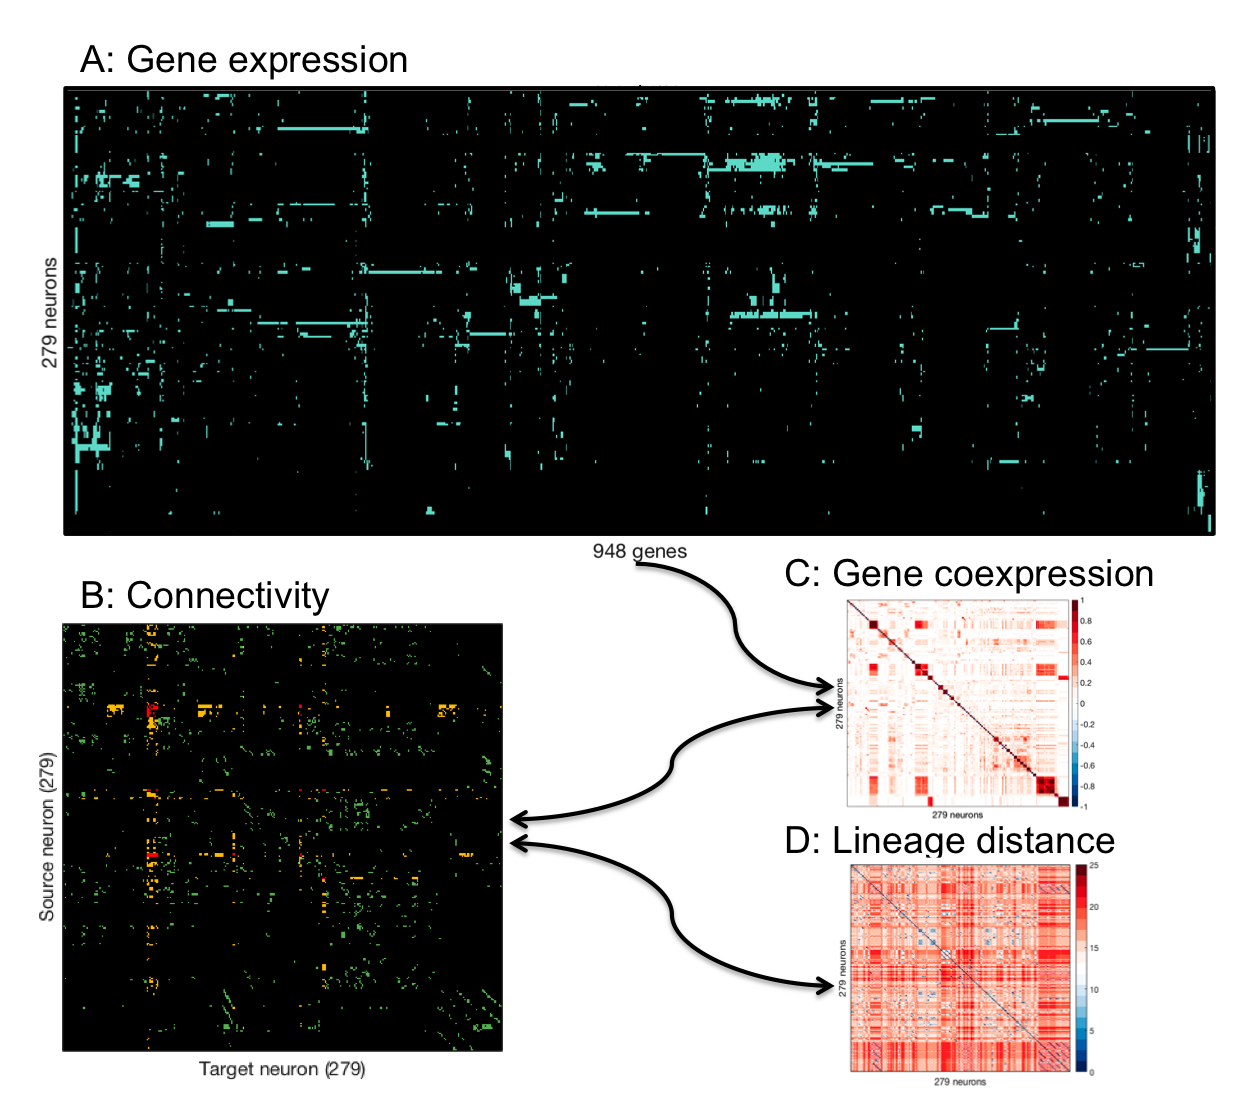
\includegraphics[width=1\textwidth]{SchematicDATA}
 \caption{{\bf Schematic representation of the work-flow}
Connectivity matrix coded according to link type (and probably gene expression matrix: rows as it is (neuron order), columns ordered according to similarity).}
 \label{fig:SchematicRepresentation}
 \end{figure}

% METHODS: gene enrichment
\subsection*{Gene enrichment analysis}
In order to interpret differences in gene coexpression between different types of node pairs, we used enrichment analysis to identify functionally annotated groups of genes from the Gene Ontology (GO) \cite{Ashburner2000}.
%  that contribute to the increased coexpression between:
% (i) connected pairs of neurons as compared to unconnected pairs as well as
% (ii) connections involving hubs (rich and feeder) compared to connections that do not involve hubs (peripheral).

Following previous work \cite{Fulcher:2016ck}, we first assigned a gene coexpression contribution (GCC) score to each gene, $g_{ij},$ that quantifies the contribution of each gene to the coexpression score for a given pair of brain regions ($i$ and $j$).

First, for each gene we determined the pattern of matching expression profiles (a match meaning that a gene is expressed by both neurons) between each pair of neurons resulting in a binary 279 x 279 matrix.
Then, for each gene we calculated a cumulative binomial probability of getting more matches $(X)$ than in the empirical data $(m)$ on a particular connection type (see eq. \ref{eq:CBinomialProbability}).
Depending on the connection type in question this can be phrased in two following ways: (i) what is the probability to get more matches on connected links given the number of connected links; (ii) what is the probability to get more matches on links involving hubs (rich and feeder) given the number of matches on connected links.
\begin{eqnarray}
	\label{eq:CBinomialProbability}
     \mathrm{P(X>m)} = 1 - \sum_{\textit{i}=0}^{m}\binom{n}{i} p^{\textit{i}}(1-p^{n-\textit{i}}),
\end{eqnarray}
where m - the number of matches in empirical data, \textit{p} - the probability of randomly choosing a selected type of connection and \textit{n} - a maximum number of possible matches given the connection type in question.


When calculating GCC for connected links more then one match for a gene overall was required (as a result 577 genes out of 948 left); when calculating GCC for the links involving hubs (rich and feeder links) more than one match was required on connected links (as a result 390 out of 948 genes left).
Otherwise, no information about the contribution of a specific gene to the overall coexpression pattern could be extracted.
\textbf{(NOTE: not literally true as both on and off matches equally contribute to an increase in coexpression, - need to find a way how to explain, why non-expression matches are not taken into account here).}\\
These GCC scores were then used to perform gene score resampling (GSR) analysis, which examines if genes with low GCC scores are statistically over-represented in any functional category.

The above mentioned analysis was done using 3.0.2 of ErmineJ \cite{Gillis2010}.
Gene annotations were assigned from GO \cite{Ashburner2000} using an annotation file from GEMMA \cite{Zoubarev2012}.
Generic\textunderscore worm \textunderscore noParents.an.txt.gz downloaded using a build-in option within ErmineJ software on February 10 2017.
GO terms and definitions were obtained in RDF XML file format downloaded from \url{archive.geneontology.org/latest-termdb/go_daily-termdb.rdf-xml.gz} on February 10 2017.
In the analysis we were considering gene set sizes in the range 5–100, taking the mean score in a GO group to summarize it.
% {archive.geneontology.org/latest-termdb/go \textunderscore daily-termdb.rdf-xml.gz}
Full resampling with $10^{7}$ iterations was used.

\textbf{Lineage distance.}\\

\textbf{Non-overlapping modules.}\\

\textbf{Overlapping modules.}



% Place figure captions after the first paragraph in which they are cited.
% \begin{figure}[!h]
% \caption{{\bf Bold the figure title.}
% Figure caption text here, please use this space for the figure panel descriptions instead of using subfigure commands. A: Lorem ipsum dolor sit amet. B: Consectetur adipiscing elit.}
% \label{fig1}
% \end{figure}

% Results and Discussion can be combined.
\section*{Results}

%%
\subsection*{Coexpression and connectivity}

%% for now figres are old - just to define where the figure is
First, we investigated how gene coexpression relates to connectivity by examining it between connected and unconnected neuron pairs.
As it is shown in Fig \ref{fig:ConUncon}, connected pairs of neurons have more similar expression profiles than unconnected pairs (Wilcoxon rank-sum test, $P < 10^{-50}$). Furthermore, there is no difference in gene coexpression between reciprocally and unidirectionally connected neurons while coexpression in both of these groups is higher than between unconnected neurons (see Fig \ref{S1_Fig}). \\

\begin{figure}[!h]
   \centering
    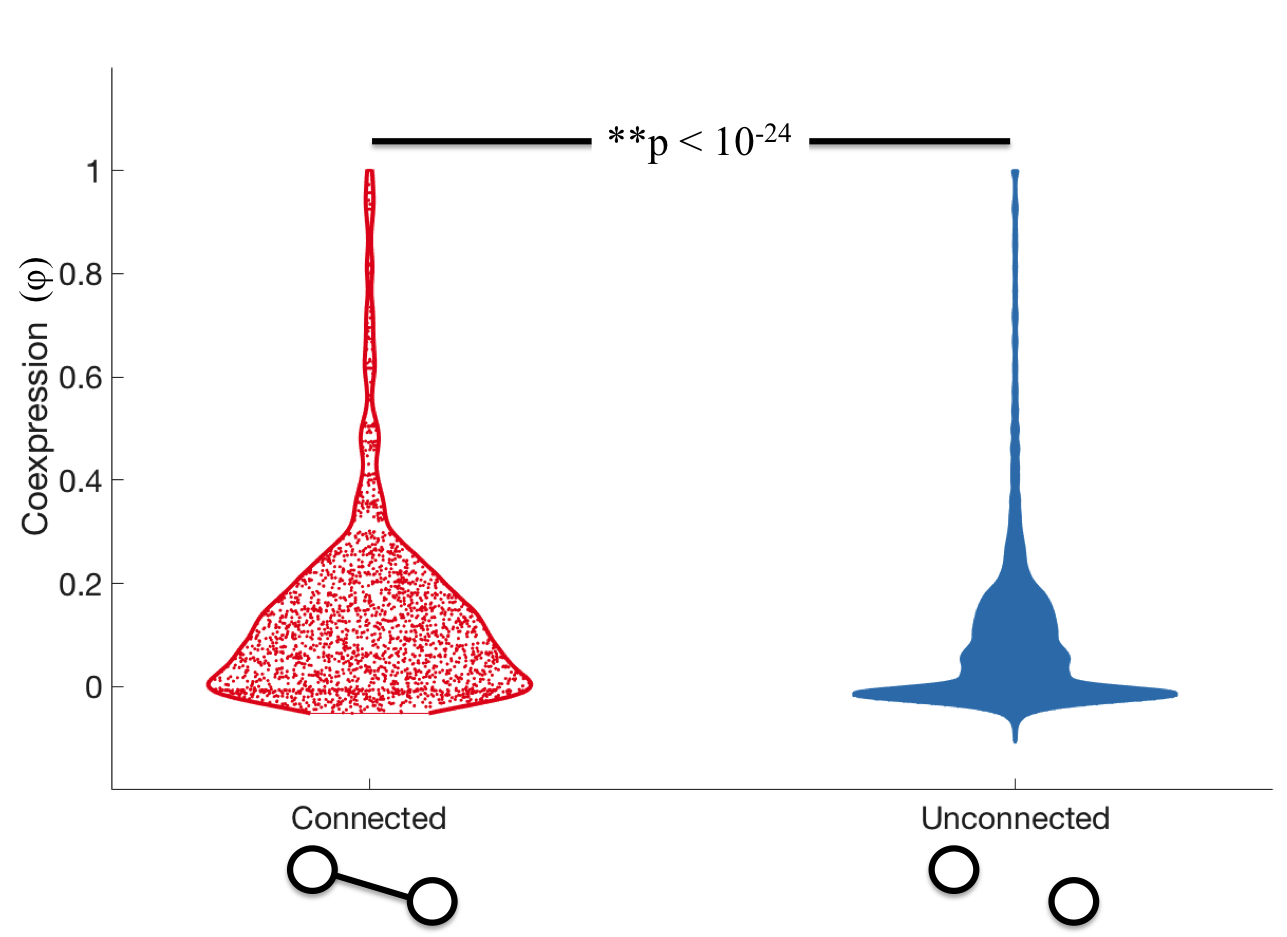
\includegraphics[width=0.9\textwidth]{ConUnconChemicalFINAL}
 \caption{{\bf Coexpression between connected and unconnected neurons.}
Distribution of transcriptional similarity between connected and unconnected neurons.
P-values are from Wilcoxon rank sum test.}
 \label{fig:ConUncon}
\end{figure}
To investigate which functional groups of genes contributed to the difference in transcriptional coupling between connected and unconnected neurons, we used a method of assigning each gene coexpression contribution (GCC) score that quantifies the contribution of each gene to the overall coexpression between neuron pairs (see Methods).  \\

%% comment on enrichment analysis. No write up can be done before deciding on options.
\textbf{NOTE: Do GRS in all cases - exclude genes with $<=$ 1 matches (genes with 1 match introduce more noise then effect) on the mask.
Enrichment results depend on the size of gene sets selected: \\
5-100 give same results for both connected and rich-feeder (glutamate plus connectivity)\\
10-100 give only one category for connected (basic connectivity) and more of the same stuff for rich and feeder (no glutamate as glutamate category is a small one).
We get sensible results only when -log(score) option is selected.
Otherwise connected links get sensory categories related to light detection.}.

The majority of the significant ($P < 0.05$) GO categories are related to neuronal connectivity and communication, as listed in Table~\ref{table1} (1st column: GO category).
These findings are in line with our expectations as they confirm that genes that are more likely to be expressed in a pair of connected neurons are in fact related to neuronal connectivity and communication.\\
\textbf{NOTE: As coexpression is increased in for both ``on'' and ``off'' matches, we might present a list for enrichment in 2 cases: ON matches (genes, that need to be both on to increase coexpression for a certain group of links), OFF matches (genes that need to be both off to increase coexpression for a certain group of links).
Would separate meaning of ON and OFF and wouldn't mislead the reader. }



%%
\subsection*{Properties of hub connectivity}
%% INTRODUCE RICH CLUB  hene and focus on the difference between rich/feeder/peripheral links below
\textbf{Rich club organization of the connectome}\\

In connectomes across species and scales, degree is distributed unequally, with a small number of highly connected brain regions, known as hubs \cite{Sporns:2007ea}, that are themselves more densely connected between themselves, forming a so-called `rich club' \cite{deReus:2013cy, ZamoraLopez:2010hy, Shih:2015cu, vandenHeuvel:2012kh, vandenHeuvel:2011he}.
The same is true in the C. elegans neuronal nervous system, analyzed in the past as an undirected binary connectome including both chemical and electrical synapses \cite{Towlson:2013gf}, which exhibits highly connected, and densely interconnected hub neurons.
As 


The extended tail of the degree distribution presented in \ref{fig:SchematicRepresentation} indicates the existence of a small number of highly connected nodes.
At each degree \textit{k} nodes in the network were classified as hubs (degree $>\textit{k}$) or non-hubs (degree $\leq\textit{k}$) and consequently all links between them separated into three categories: rich (hub $\rightarrow$ hub), feeder (hub $\rightarrow$ non-hub or non-hub $\rightarrow$ hub) and peripheral (non-hub $\rightarrow$ non-hub).


In this work we use a directed binary connectivity matrix of chemical synapses provided by \citet{Varshney2011} for 279 non-pharingeal neurons (nodes) and 1961 connections between them (edges) and show a rich-club organisation of the chemical synapse network (see \textit{Materials and Methods}).
Rich-club organisation manifests across a continuous range of degrees $41<k<58$ ($P<0.05$, shaded grey area in Fig.\ref{RCcoef}) as normalised rich-club coefficient $\Phi_{norm}>1$.
This indicates that when nodes are defined as hubs (degree $>\textit{k}$) in this range, they are more densely interconnected than expected by chance.
Rich club in the chemical synapse network consists of 13 high degree neurons with degree $42 \leq k \leq 98$. \\
\textbf{(NOTE: maybe include a list with degrees and definitions in SUPP (like in Towlson's paper?)).}

\begin{figure}[!h]
   \centering
    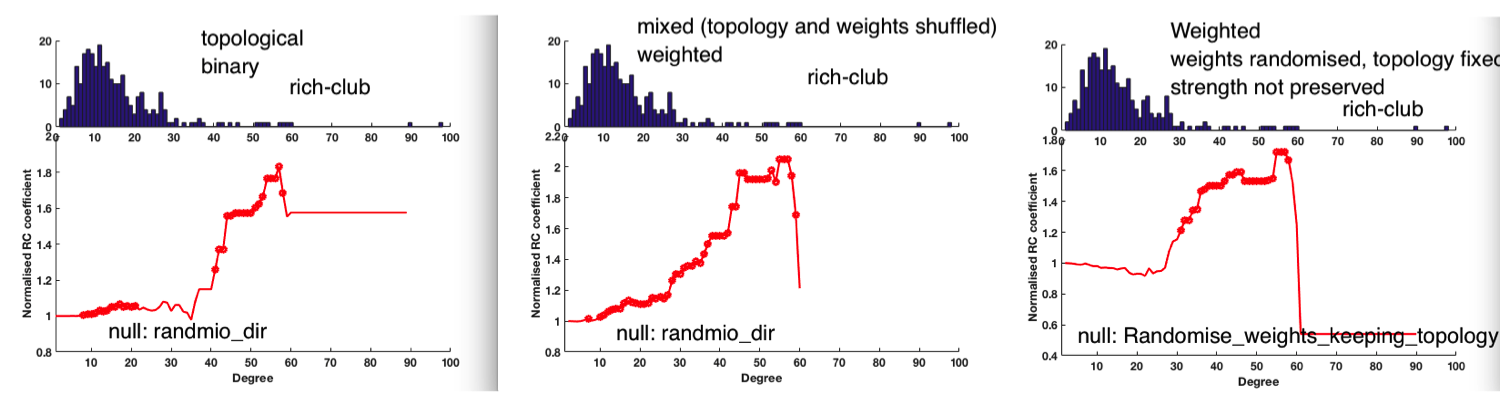
\includegraphics[width=1\textwidth]{RCcurveFINAL3}
 \caption{{\bf Rich-club organisation of the connectome.} \\
A: Topological rich-club. B: Mixed rich-club. C: Weighted rich-club. \\
Normalized rich club coefficient, $\Phi_{random}$ as a function of the degree, \textit{k}, at which hubs (regions with degree $\geq \textit{k}$) are defined. (permutation test; $P<0.05$).
$\Phi_{norm}>1$ indicates that hubs are more densely interconnected among each other than expected by chance.
Red circles indicate values of $\Phi_{random}$ that are significantly higher than an ensemble of 1000 null networks.\\
\textbf{NOTE: plot three curves in one plot (with different colours) and shade grey the overlapping area. } }
 \label{RCcoef}
 \end{figure}


\textbf{Coexpression and hub connectivity.}\\
For the second part of our analysis, we focused on the features of rich-club organization of \textit{C. elegans} connectome by investigating the relationship between gene coexpression and neuronal connectivity in three different classes of neuron pairs.
At each node degree, $k$ (x-axis in Fig \ref{RCdegree}), we defined each neuron as either a hub (nodes with degree $\geq k$) or a nonhub (otherwise), and then labelled each connection as rich (hub $\rightarrow$ hub), feeder (nonhub $\rightarrow$ hub or hub $\rightarrow$ nonhub), or peripheral (nonhub $\rightarrow$ nonhub).
Then at each degree, we calculated median coexpression values for each link type (Fig. \ref{RCdegree}).
Median was chosen instead of the mean due to non-normal coexpression value distributions.
Coexpression is gradually increasing with degree for links involving hubs (Fig. \ref{RCdegree}).
Rich links show consistently increasing coexpression for a range of degrees until it reaches plateau at around $k=38$ and stays constant in the topological rich club regime.
Median coexpression also increases slightly for feeder links from around the same threshold $k=38$, while pthe curve for peripheral links remain flat through the range of degrees.

 \begin{figure}[!h]
 \centering
    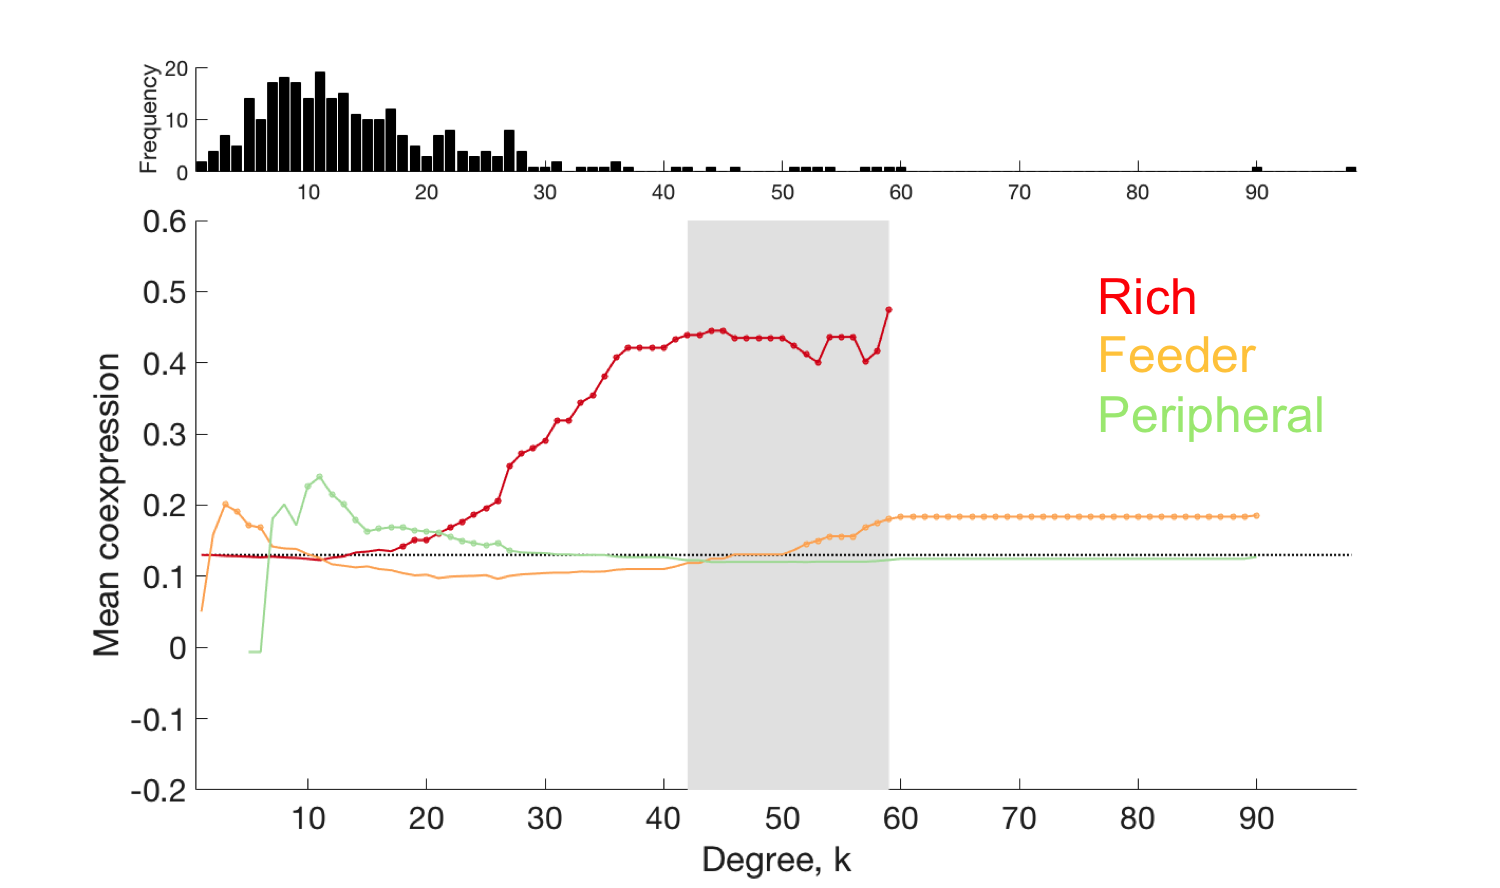
\includegraphics[width=0.7\textwidth]{RichFeederPeripheral_k}
 \caption{{\bf Mean coexpression for rich, feeder and peripheral links as a function of degree.}
Top: degree distribution. Median gene coexpression for rich, feeder, and peripheral connections as a function of \textit{k}, with the median across all network links shown as a dashed black line and the topological rich club regime shaded grey.
Circles indicate a statistically significant increase in gene coexpression in a given link type relative to the rest of the network (Wilcoxon rank sum test; $P < 0.05$)}
 \label{RCdegree}
 \end{figure}


\begin{figure}[!h]
 \centering
    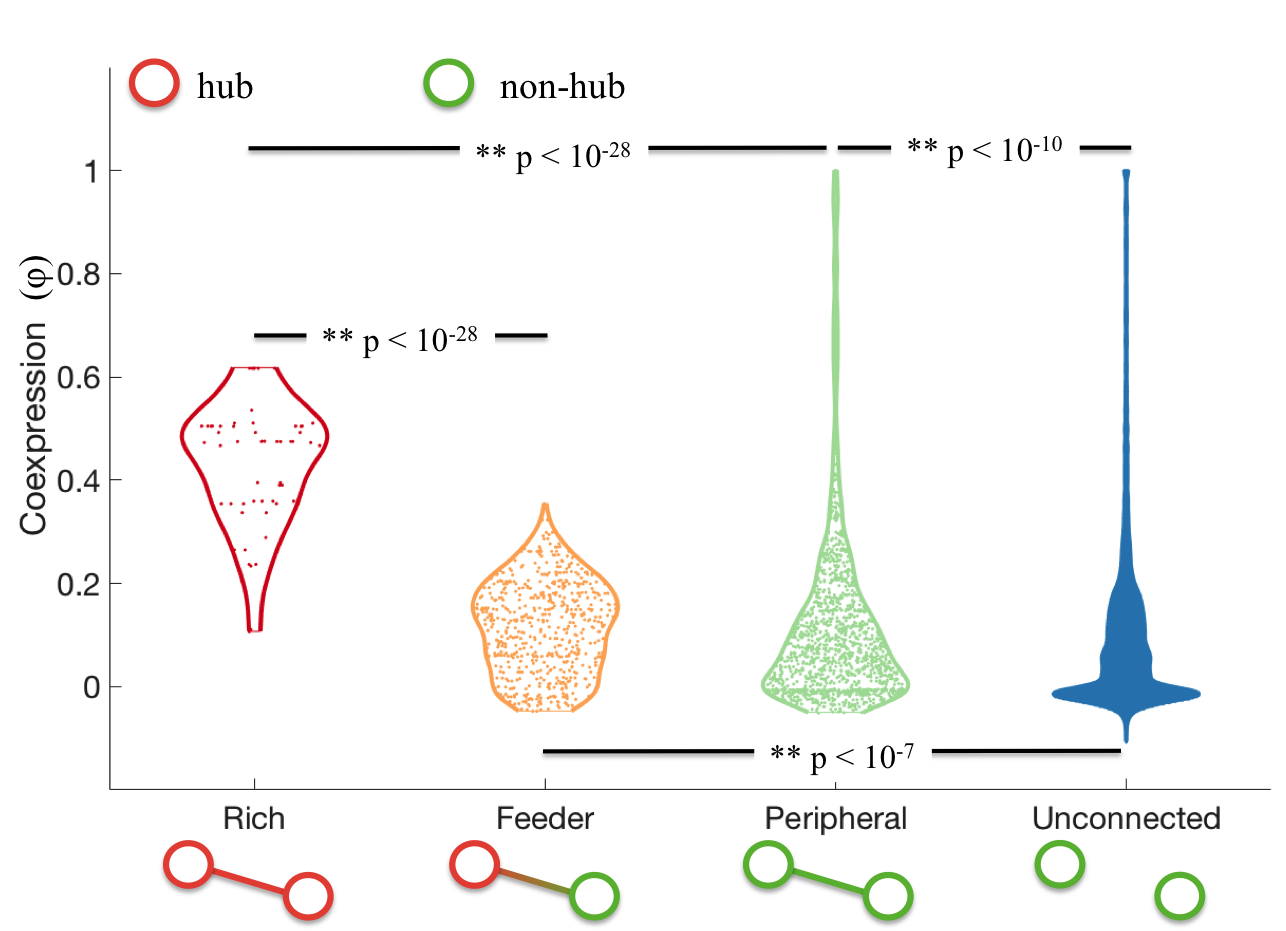
\includegraphics[width=1\textwidth]{RichFeederPeripheral_k42FINAL}
 \caption{{\bf Coexpression for rich, feeder and peripheral links as a function of degree.}
Coexpression ($\phi$) for different types of network connections, where hubs are neurons with degree $k \geq 42$. P-values are from Wilcoxon rank sum test. \\
SHOW THIS IN SUPP}
 \label{ViolinPlots}
 \end{figure}

To investigate which functional groups of genes contributed to the increased coexpression for links involving hubs (rich and feeder) we used a method of assigning each gene a GCC measure that quantifies the contribution of each gene (see Methods).

Enrichment analysis show that the majority of the significant ($P < 0.05$) GO categories are related to glutamate signalling, neuronal connectivity and communication.
It is line with the previous analysis where same GO categories were shown to be significant in differentiating connected from unconnected neurons. 
%% combine enrichment tables into one
\begin{table}[!ht]
\begin{adjustwidth}{-2.25in}{0in} % Comment out/remove adjustwidth environment if table fits in text column.
\centering
\caption{
{\bf Enrichment.}}
\begin{tabular}{ |c|c|c|c| }
\thickhline
\multicolumn{2}{c}{Connected \textit{vs} unconnected} & \multicolumn{2}{c}{Rich and feeder \textit{vs} peripheral} \\ \hline
%{\bf Connected} & {} & {\bf Rich and feeder}\\ \thickhline
GO category  & pvalue & GO category  	& p value \\ \thickhline
glutamate receptor signalling pathway 	& $10^{-7}$ 	& glutamate receptor signalling pathway 			& $10^{-5}$\\ \hline
ionitropic glutamate receptor signalling	& $10^{-7}$ 	& ionitropic glutamate receptor signalling		& $10^{-5}$ \\ \hline
synaptic transmission, glutamatergic 	& $10^{-7}$	& synaptic transmission, glutamatergic 			& $10^{-5}$ \\ \hline
neuron-neuron synaptic transmission 		& $10^{-5}$	& chemical synaptic transmission	 	 			& $10^{-5}$\\ \hline
chemical synaptic transmission		 	& 0.00057 	& anterograde trans-synaptic signalling			& $10^{-5}$\\ \hline
anterograde trans-synaptic signalling 	& 0.00057 	& synaptic signalling 							& $10^{-5}$\\ \hline
synaptic signalling 						& 0.00057 	& trans-synaptic signalling	 					& $10^{-5}$\\ \hline
trans-synaptic signalling				& 0.00057 	& neuron-neuron synaptic transmission  			& 0.00031 \\ \hline
										&  			& cell-cell signalling				  			& 0.00086 \\ \hline
										&  			& cell surface receptor signalling pathway 		& 0.00107 \\ \hline
\end{tabular}
\begin{flushleft} Table notes what GO categories were overrepresented in driving the difference between different types of links.
\end{flushleft}
\label{table1}
\end{adjustwidth}
\end{table}

These findings are in line with our expectations as high degree neurons are highly involved in signalling and the majority of hubs while being cholinergic, receive input from sensory neurons the majority of which is glutamatergic. \\
NOTE: NOTE HERE ABOUT REDUCED LIST OF GENES IN EACH ANALYSIS (577 and 390 genes for connected and R/F respectively) AND WHAT IMPACT THAT COULD HAVE ON RESULTS.

\subsection*{EXTRAS}
\begin{itemize}
    \item{Difference between interneurons/motor/sensory neurons - effect driven by interneurons}
    \item{Maybe include lineage data: lineage distance increases with degree for feeder links; no difference between rich and peripheral links; Sort of confirms separation into rich/feeder/peripheral links as distance increases for feeders?}
\end{itemize}
\subsection*{Neuron type}
While above we demonstrated a relationship between transcriptional similarity and structural connectivity, we note that all hubs in the topological rich-club regime in the C. elegans connectome are interneurons.
Correspondingly, we investigated whether the effect of increasing gene coexpression is specific to interneurons.
The relationship between median coexpression and degree for connections including different types of neurons (interneurons, motor neurons and sensory neurons) is shown in Fig. \ref{NeuronTypePlot}.
Connections involving interneurons show a pattern of increasing average coexpression with increasing degree, however neither connections involving motor nor sensory neurons resemble this trend; even showing evidence for the opposite relationship.
In other words, motor and sensory neurons with higher degree show less similar gene expression patterns.

\begin{figure}[!h]
\centering
    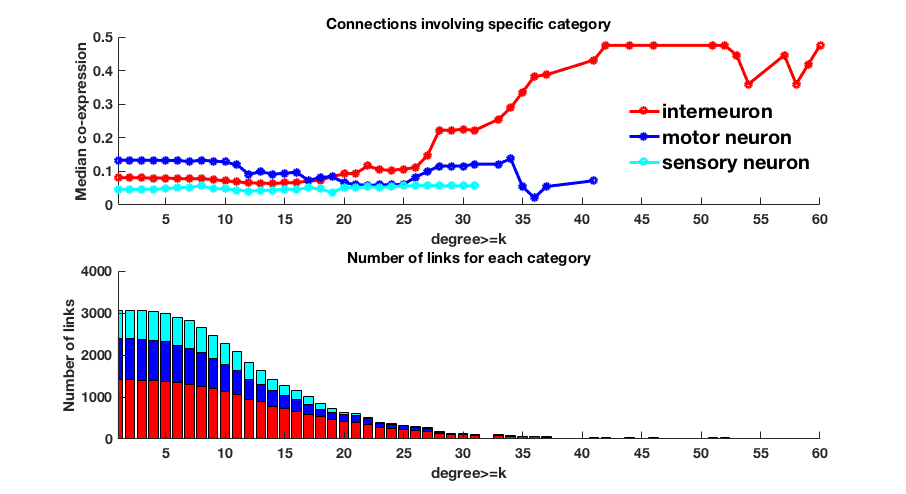
\includegraphics[width=1\textwidth]{coexpressionInvolvingCategory}
 \caption{{\bf Coexpression for different types of neurons. }
Top: Average gene coexpression as a function of degree for connections involving different types of neurons. Bottom: The number of connections in each category for a range of degrees.}
 \label{NeuronTypePlot}
 \end{figure}
Top: Average gene coexpression as a function of degree for connections involving different types of neurons. Bottom: The number of connections in each category for a range of degrees.

Next, we compare transcriptional similarity between hub interneurons and non-hub interneurons that share similar anatomical properties.
\textbf{Compare coexpression between hub interneurons and non-hub interneurons with the same anatomy here.}
\subsection*{Lineage}
\begin{figure}[!h]
\centering
    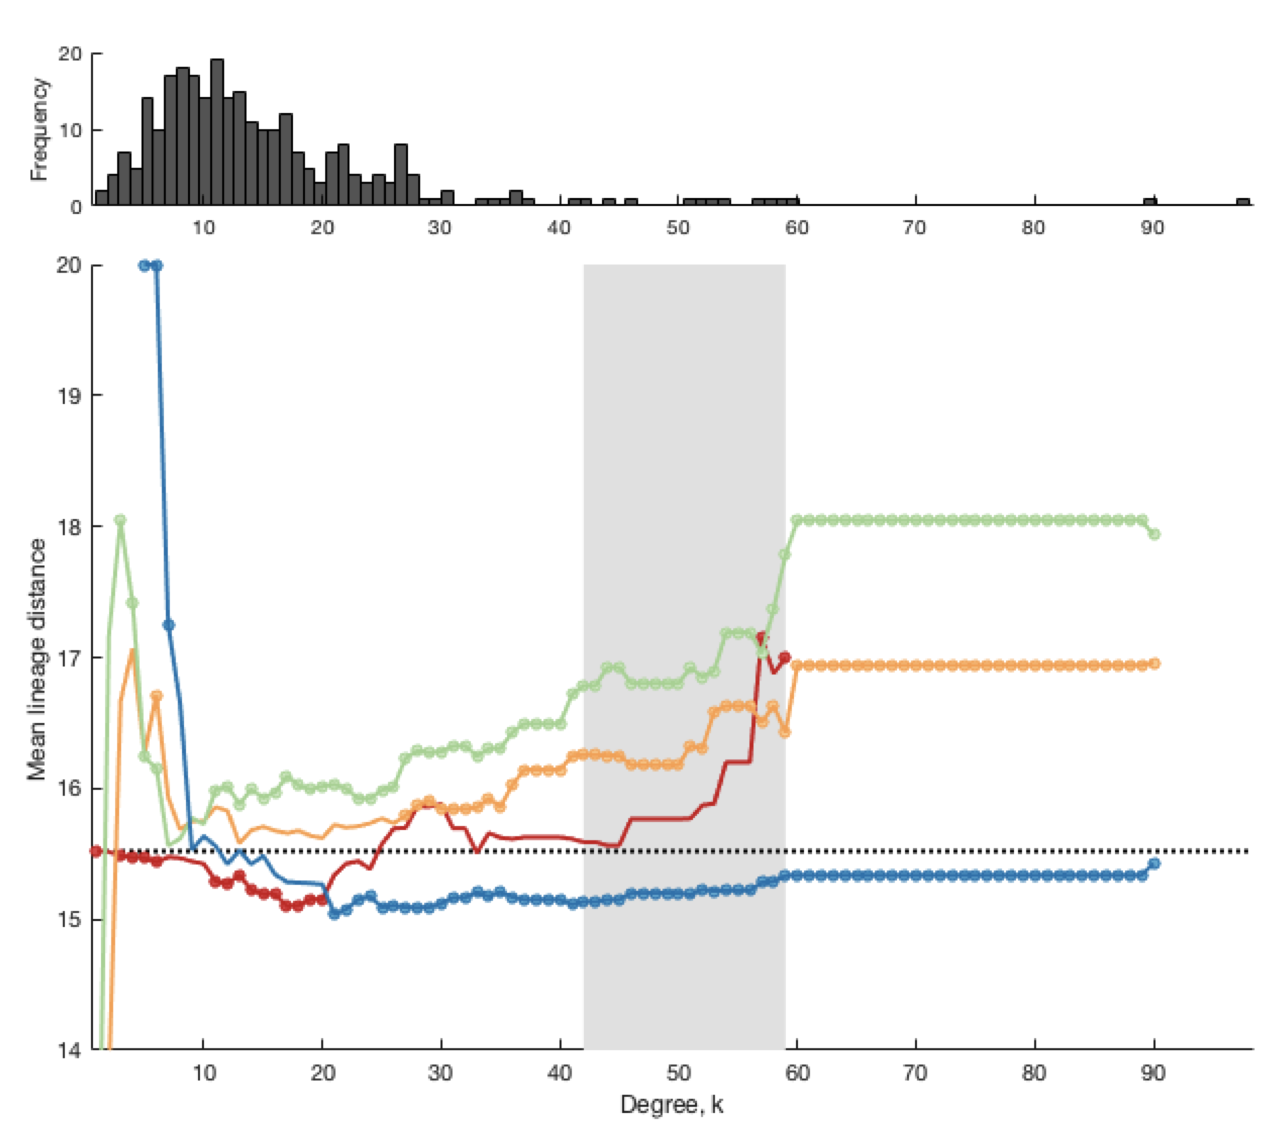
\includegraphics[width=1\textwidth]{LineageRFP}
 \caption{{\bf Coexpression for different types of neurons. }
Top: Average gene coexpression as a function of degree for connections involving different types of neurons. Bottom: The number of connections in each category for a range of degrees. }
 \label{Lineage}
 \end{figure}
\subsection*{Modules}
\textbf{Chemical BINARY}\\
Changing tau value can get from 4 to 6 modules:\\
4 modules: \\
* 95\% of RC links are within one module (module 3), which is dominated by motor neurons \\
* 5\% RC links within module 2 \\
No RC links between modules. \\
module 4 - small motor neuron module. \\

5 modules: \\
trends the same, 2 small modules originates. \\
all RC links are within modules. \\

6 modules:\\
* 45 \% RC links within module 3\\
* 5 \% and 5 \% RC links in modules 2 and 4.
Major module (module 3) dominated by motor neurons.
around 45 \% RC links connect different modules. \\
as the number of modules increases, more RC links tend to connect different modules between themselves (instead of connecting nodes within a module) \\
Modules with the most of RC links have highest coexpression despite having longest connection distances.

\begin{figure}[!h]
\centering
    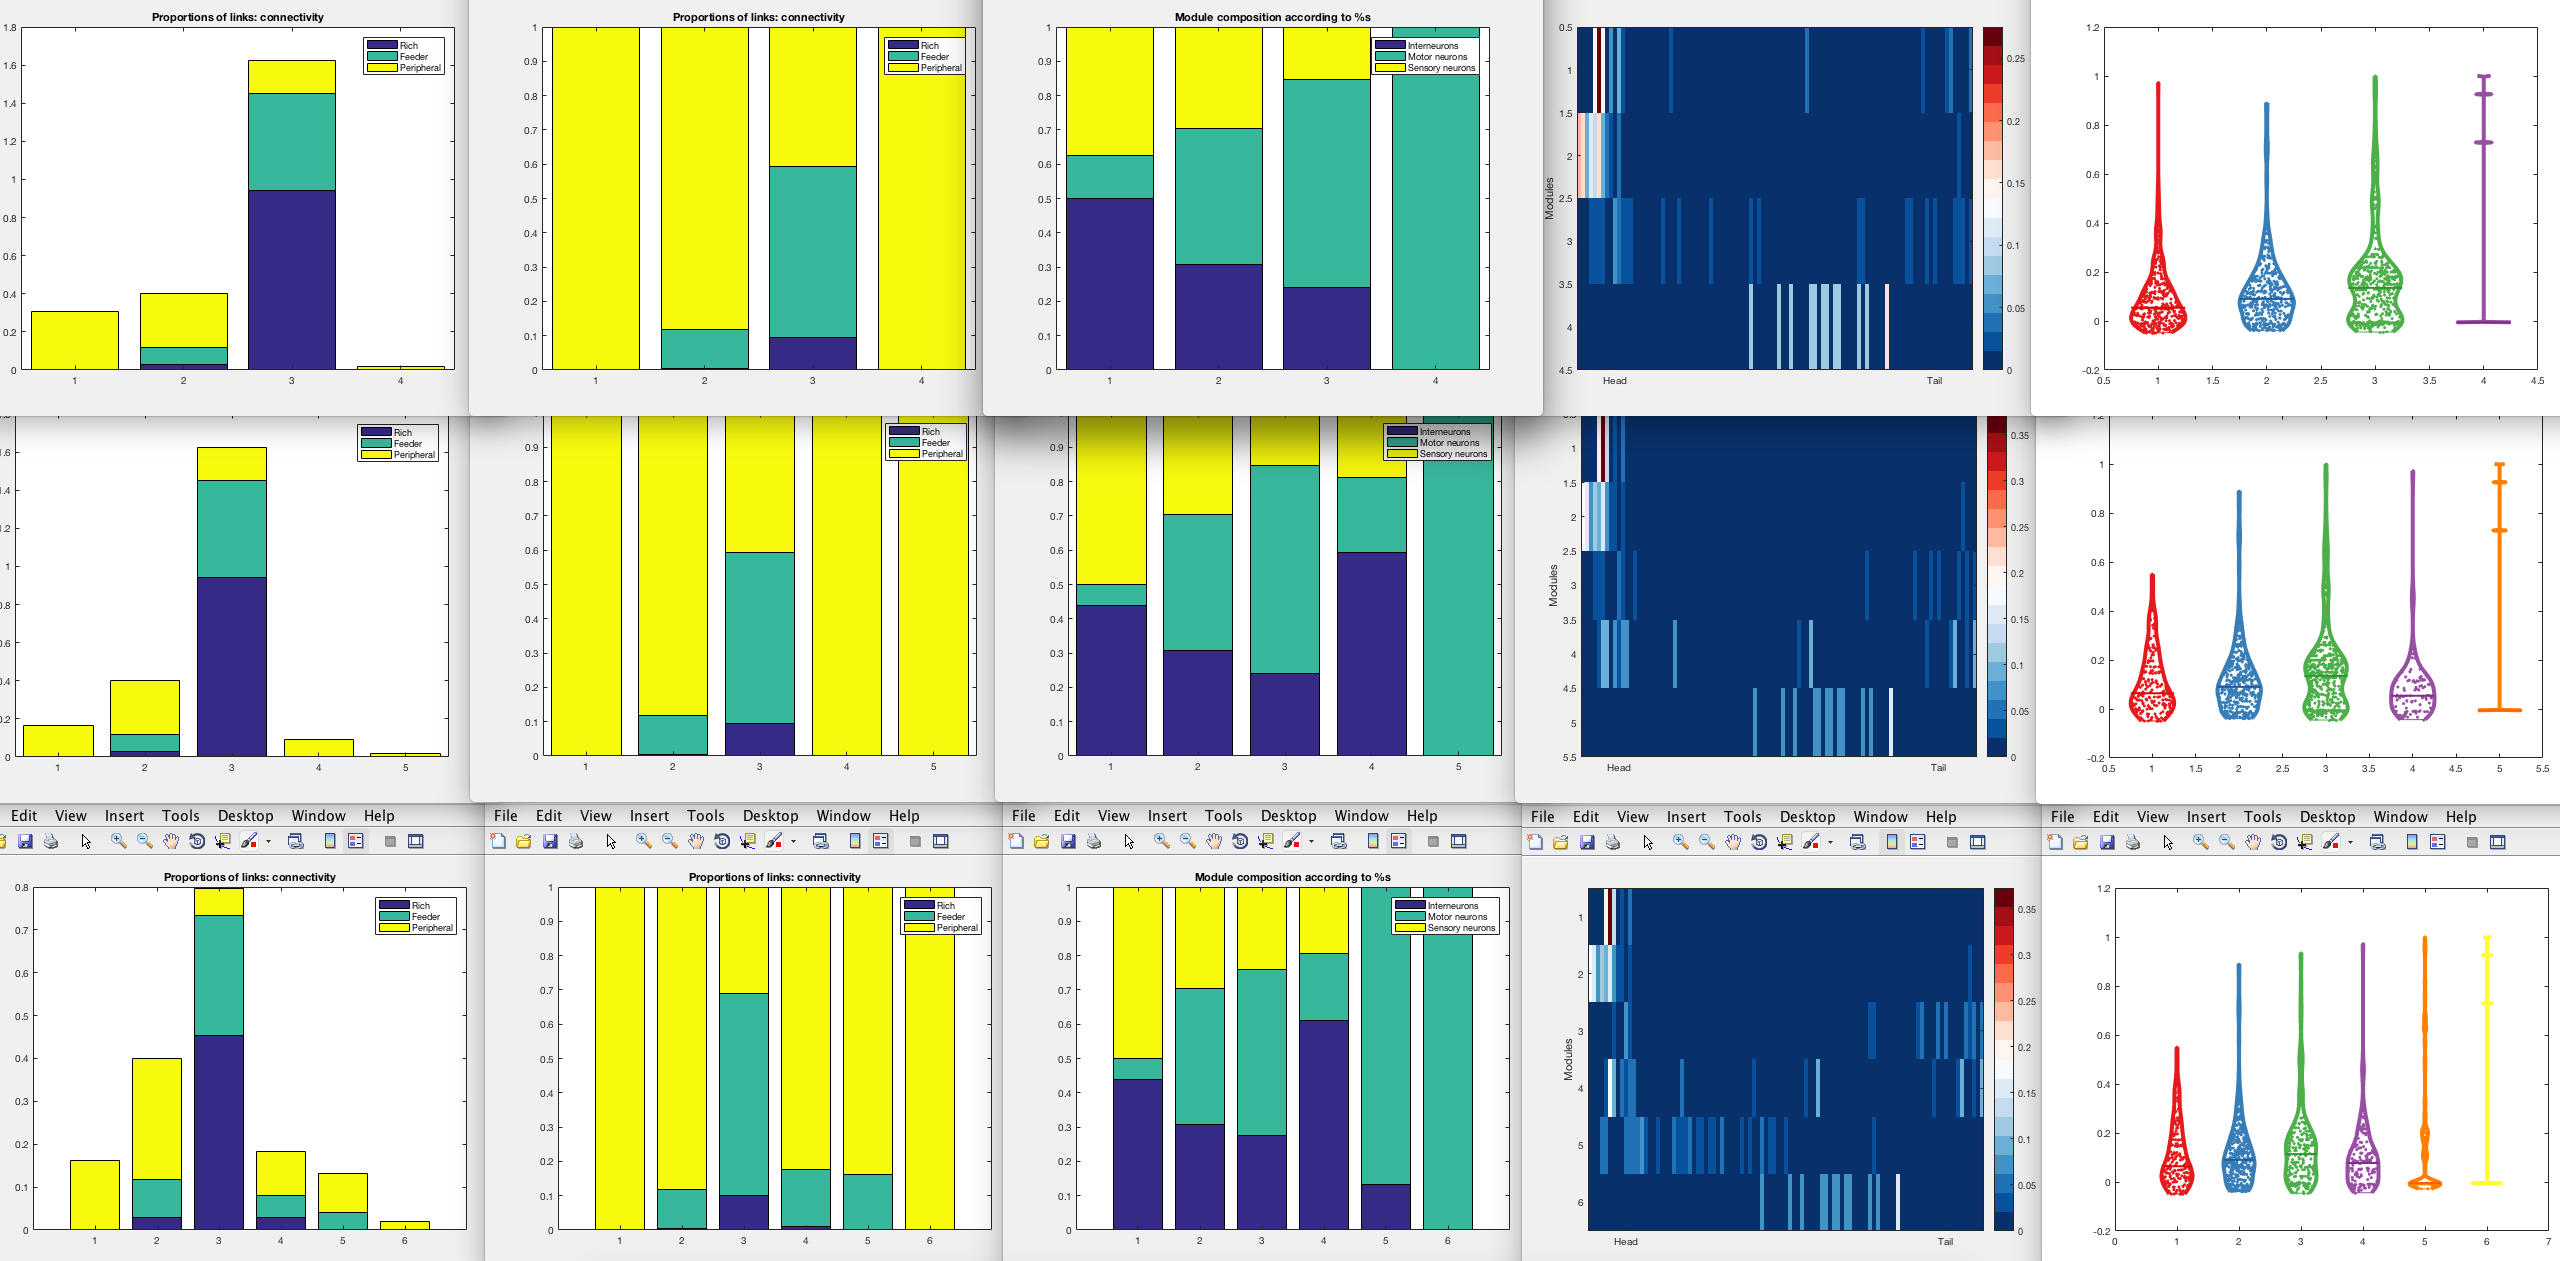
\includegraphics[width=1\textwidth]{modules}
 \caption{{\bf Modular compositions}
1st row: 4 modules (tau=0.2). 2nd row: 5 modules (tau=0.3). 3rd row (tau=0.5). }
 \label{Modules}
 \end{figure}

\textbf{Chemical WEIGHTED}\\
for a range of tau thresholds (0.1-0.5), same result: \\
7 modules. \\
* 60\% RC links are within module 1\\
* 5\% RC links are within module 3\\
* 35 \% of RC links connect different modules between themselves. \\

There are four really small modules, three of them purely motor neuron modules (5.6.7).
Module 1 - high proportion of motor neurons! module distributed through the body.
around 50 \% of feeder links link different modules; another half link nodes within 1 and 4 modules.
Module 1 has highest coexpression despite having highest connection cost (longest distances)




%%

% Place tables after the first paragraph in which they are cited.
% \begin{table}[!ht]
% \begin{adjustwidth}{-2.25in}{0in} % Comment out/remove adjustwidth environment if table fits in text column.
% \centering
% \caption{
% {\bf Table caption Nulla mi mi, venenatis sed ipsum varius, volutpat euismod diam.}}
% \begin{tabular}{|l+l|l|l|l|l|l|l|}
% \hline
% \multicolumn{4}{|l|}{\bf Heading1} & \multicolumn{4}{|l|}{\bf Heading2}\\ \thickhline
% $cell1 row1$ & cell2 row 1 & cell3 row 1 & cell4 row 1 & cell5 row 1 & cell6 row 1 & cell7 row 1 & cell8 row 1\\ \hline
% $cell1 row2$ & cell2 row 2 & cell3 row 2 & cell4 row 2 & cell5 row 2 & cell6 row 2 & cell7 row 2 & cell8 row 2\\ \hline
% $cell1 row3$ & cell2 row 3 & cell3 row 3 & cell4 row 3 & cell5 row 3 & cell6 row 3 & cell7 row 3 & cell8 row 3\\ \hline
% \end{tabular}
% \begin{flushleft} Table notes Phasellus venenatis, tortor nec vestibulum mattis, massa tortor interdum felis, nec pellentesque metus tortor nec nisl. Ut ornare mauris tellus, vel dapibus arcu suscipit sed.
% \end{flushleft}
% \label{table1}
% \end{adjustwidth}
% \end{table}


%PLOS does not support heading levels beyond the 3rd (no 4th level headings).

% \subsubsection*{3rd level heading}
% Text.
%
% \begin{enumerate}
%     \item{react}
%     \item{diffuse free particles}
%     \item{increment time by dt and go to 1}
% \end{enumerate}
%
%
% \subsection*{Another subsection}
%
%
% \begin{itemize}
%     \item First bulleted item.
%     \item Second bulleted item.
%     \item Third bulleted item.
% \end{itemize}

\section*{Discussion}
\begin{itemize}
    \item{First coexpression analysis in worm. Despite noisy gene expression data we get some insights into the genetic basis of connectivity on a neuronal level}
\end{itemize}
Discussion text
\section*{Limitations}

\begin{itemize}
    \item{Binary gene expression data}
    \item{No way of discriminating between missing data and the absence of expression}
    \item{only around 5 percent of genes in the genome available}
    \item{annotation problems: different qualifiers, loosing sensitivity/specificity if including too much or too little - need to balance}

\end{itemize}

\section*{Conclusion}

Conclusion text.

\section*{Supporting information}

% Include only the SI item label in the paragraph heading. Use the \nameref{label} command to cite SI items in the text.
\paragraph*{S1 Fig.}
{\bf Coexpression between reciprocally connected, unidirectionally connected and unconnected neurons.} P-values are from Wilcoxon rank sum test.
\begin{figure}[!h]
\label{S1_Fig}
\centering
    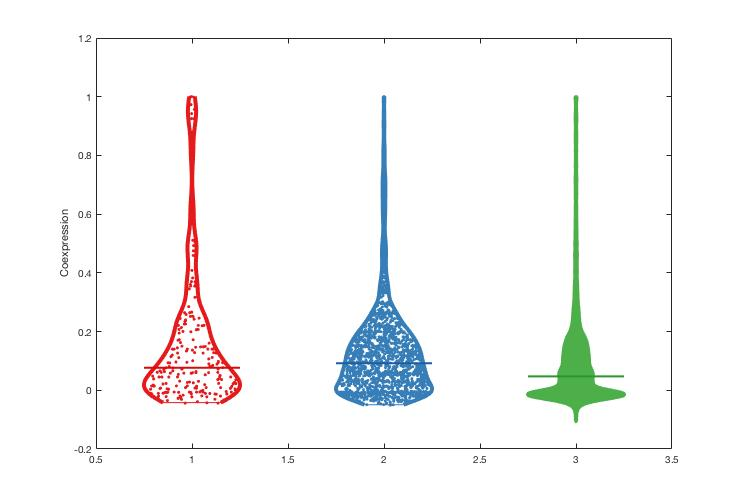
\includegraphics[width=1\textwidth]{RecUnidirUncon}
\end{figure}


\paragraph*{S2 Fig.}
\label{S2_Fig}
{\bf Lorem ipsum.} Maecenas convallis mauris sit amet sem ultrices gravida. Etiam eget sapien nibh. Sed ac ipsum eget enim egestas ullamcorper nec euismod ligula. Curabitur fringilla pulvinar lectus consectetur pellentesque.

\paragraph*{S1 File.}
\label{S1_File}
{\bf Lorem ipsum.}  Maecenas convallis mauris sit amet sem ultrices gravida. Etiam eget sapien nibh. Sed ac ipsum eget enim egestas ullamcorper nec euismod ligula. Curabitur fringilla pulvinar lectus consectetur pellentesque.

\paragraph*{S1 Video.}
\label{S1_Video}
{\bf Lorem ipsum.}  Maecenas convallis mauris sit amet sem ultrices gravida. Etiam eget sapien nibh. Sed ac ipsum eget enim egestas ullamcorper nec euismod ligula. Curabitur fringilla pulvinar lectus consectetur pellentesque.

\paragraph*{S1 Appendix.}
\label{S1_Appendix}
{\bf Lorem ipsum.} Maecenas convallis mauris sit amet sem ultrices gravida. Etiam eget sapien nibh. Sed ac ipsum eget enim egestas ullamcorper nec euismod ligula. Curabitur fringilla pulvinar lectus consectetur pellentesque.

\paragraph*{S1 Table.}
\label{S1_Table}
{\bf Lorem ipsum.} Maecenas convallis mauris sit amet sem ultrices gravida. Etiam eget sapien nibh. Sed ac ipsum eget enim egestas ullamcorper nec euismod ligula. Curabitur fringilla pulvinar lectus consectetur pellentesque.

\section*{Acknowledgments}
Thanks to Alex Fornito, for being a big deal.\\
Should keep this!
\nolinenumbers

% Either type in your references using
% \begin{thebibliography}{}
% \bibitem{}
% Text
% \end{thebibliography}
%
% or
%
% Compile your BiBTeX database using our plos2015.bst
% style file and paste the contents of your .bbl file
% here. See http://journals.plos.org/plosone/s/latex for
% step-by-step instructions.
%

\bibliography{library,library_ben}
% \begin{thebibliography}{10}

% \bibitem{bib1}
% Conant GC, Wolfe KH.
% \newblock {{T}urning a hobby into a job: how duplicated genes find new
%   functions}.
% \newblock Nat Rev Genet. 2008 Dec;9(12):938--950.
%
% \bibitem{bib2}
% Ohno S.
% \newblock Evolution by gene duplication.
% \newblock London: George Alien \& Unwin Ltd. Berlin, Heidelberg and New York:
%   Springer-Verlag.; 1970.
%
% \bibitem{bib3}
% Magwire MM, Bayer F, Webster CL, Cao C, Jiggins FM.
% \newblock {{S}uccessive increases in the resistance of {D}rosophila to viral
%   infection through a transposon insertion followed by a {D}uplication}.
% \newblock PLoS Genet. 2011 Oct;7(10):e1002337.

% \end{thebibliography}



\end{document}
